\subsection{Theory}

\subsubsection{Noise}

One of the most funadmental tools used in PCG is noise.
Noise is the concept of random values, often represented using a 2D or 3D matrix of real numbers.
The two major types of noise that are commonly used are \textit{value noise} and \textit{gradient noise}.

\textit{Value noise} is constructed by first randomizing the values of a few lattice points in the matrix, and then interpolating these values for intermediate points.
Bilinear and bicubic interpolation are common in practice since they are fast to compute.
Value noise is simple to implement, but it has several disadvantages.
First off, the noise ends up with a grid-like structure because of the lattice points.
This is often undesired since it creates arbitrary patterns in the noise.
Furthermore, neighboring lattice points may greatly differ in values which can result in sudden changes in steepness.

\textit{Gradient noise} solves the problems with value noise by first constructing slopes, and then sample values from those.
By interpolating slopes (or gradients) that already are smooth, we ensure that not only changes in values are smooth but also the \textit{rate of change} between them.
This causes nearby points to be of similar random values, while points far apart to be unrelated.

Both types of noise can be represented with intensity maps as seen in figure~\ref{fig:noisetypes}.
An intensity map is a bitmap image where each pixel represents the value of the underlying noise.
White pixels indicate maximum values, and black pixels represents minimum values.
These maps can be used to represent many things including heights, in which case they are referred to as \textit{heightmaps}.
They can also be used to create smooth blending between textures.

\begin{figure}[h!]
  \centering

  \begin{subfigure}[b]{0.30\textwidth}
    \frame{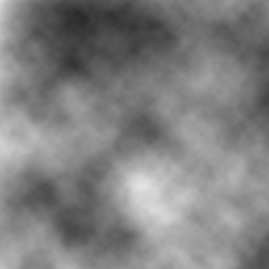
\includegraphics[width=\textwidth]{figure/value_noise.png}}
    \caption{Value noise. \cite{value_noise}}
  \end{subfigure}
  \quad
  \quad
  \quad
  % NOTE(anton): image generated from https://cpetry.github.io/TextureGenerator-Online/
  \begin{subfigure}[b]{0.30\textwidth}
    \frame{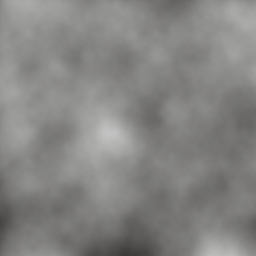
\includegraphics[width=\textwidth]{figure/heightmap.png}}
    \caption{Gradient noise.}
  \end{subfigure}

  \caption{Examples of value noise and gradient noise represented using intensity maps. Notice how the value noise has cross-like patterns.}
  \label{fig:noisetypes}
\end{figure}

A commonly used implementation of gradient noise is \textit{Perlin noise}, which later evolved into an improved version called \textit{simplex noise}.
Ken Perlin introduced \textit{Perlin noise} in 1985 with the intention to produce more natural looking textures \cite{perlin_noise}.
Although \textit{simplex noise} is the improved version, the two terms are often used interchangeably. The idea of \textit{simplex noise} is described in great detail by Stefan Gustavson in his paper \textit{Simplex noise demystified} \cite{simplex_noise}.
He also mentions several technical advantages with the technique.